\documentclass[runningheads]{llncs}
%% To switch to NeurIPS format:
%%   1. Replace \documentclass above with:
%%        \documentclass{article}
%%        \usepackage[preprint]{neurips_2026}
%%   2. Remove \institute, adjust \author
%%   3. Remove \keywords
%% The content, tables, and structure are NeurIPS-compatible as-is.

\usepackage[T1]{fontenc}
\usepackage{graphicx}
\usepackage{booktabs}
\usepackage{amsmath}
\usepackage{xcolor}
\usepackage{hyperref}

\newcommand{\method}{Envisage}
\newcommand{\best}[1]{\textbf{#1}}
\newcommand{\second}[1]{\underline{#1}}

\begin{document}

\titlerunning{Envisage: Depth-Conditioned Inpainting for Surgery Prediction}

\title{\method{}: Depth-Conditioned Diffusion Inpainting\\
for Facial Surgery Outcome Prediction}

\author{Agarwal, Mudit}
\institute{Vanderbilt University}

\maketitle

%% ========================================================================
%% ABSTRACT
%% ========================================================================
\begin{abstract}
Predicting the visual outcome of facial surgery from a single
pre-operative photograph is important for patient consent and surgical
planning, yet existing approaches either apply geometric morphing
that lacks photorealism or generate the entire face from a conditioning
signal, altering patient identity in regions the surgeon does not touch.
Here, we mask only the surgical region and modify a monocular depth map
to reflect the target tissue displacement, then use a pretrained
depth-conditioned diffusion model to regenerate the masked area. We
introduce decomposed identity evaluation, in which ArcFace cosine
similarity is measured separately on the surgical region, non-surgical
region, and full face. On the HDA Plastic Surgery benchmark (57 test
pairs, 3 procedures), \method{} achieves 0.802 ArcFace for rhinoplasty
(compared to 0.607 for a full-face diffusion baseline, +32\%) and 0.745
for blepharoplasty (+11\%), with non-surgical region ArcFace of
0.985--0.989. These results are obtained with zero task-specific
training; the pretrained depth ControlNet suffices to produce
anatomically coherent predictions from modified depth maps alone.

\keywords{Facial surgery prediction \and Diffusion inpainting \and
Depth conditioning \and Identity preservation \and Fairness}
\end{abstract}

%% ========================================================================
%% 1. INTRODUCTION
%% ========================================================================
\section{Introduction}
\label{sec:intro}

Facial plastic surgery accounts for over 15 million procedures per
year globally, with rhinoplasty and blepharoplasty among the most
requested~\cite{asps2023stats}. Patient satisfaction is strongly
associated with pre-operative expectation management; studies report
revision rates of 5--15\% for rhinoplasty, driven in part by
discrepancies between expected and actual
outcomes~\cite{honigman2004review,sarwer2008body}. Current prediction
tools range from surgeon-drawn sketches to proprietary 3D simulation
systems (Crisalix, Vectra 3D) that require dedicated hardware costing
\$30,000--50,000. No widely available system produces photorealistic
predictions from a single 2D photograph while guaranteeing that the
patient's identity is preserved in non-surgical regions.

Several approaches to automated surgical prediction have been explored.
Geometric morphing methods based on thin-plate spline (TPS)
warps~\cite{bookstein1989tps} can approximate structural changes but
introduce boundary artifacts and cannot synthesize new skin texture.
Three-dimensional approaches (ACMT-Net~\cite{li2023acmt},
Ma et~al.~\cite{ma2023gposc}) operate on CT scans or 3D meshes,
limiting their applicability to the 2D photograph setting that is
most accessible in clinical practice. Full-face diffusion models,
including our own earlier exploration with SD~1.5 conditioned on
landmark wireframes, regenerate the entire face from a structural
conditioning signal; that preliminary system achieved 0.509 ArcFace
for rhinoplasty, and analysis revealed that nearly all identity
preservation (0.509 vs.\ 0.023 without compositing) was attributable
to post-hoc pixel compositing rather than the diffusion model itself.
DragDiffusion~\cite{shi2024dragdiffusion} allows point-based image
editing but provides no procedure-specific anatomical structure.

These observations motivated a fundamental redesign. Rather than
generating the full face and compositing afterward, we formulate
surgical prediction as \emph{inpainting}: mask the surgical region,
modify the depth map to reflect the target tissue change, and let a
pretrained depth-conditioned diffusion model regenerate only the masked
area. The key insight is that depth modification (e.g., flattening the
nasal bridge depth to simulate dorsal hump reduction) provides a
physically meaningful conditioning signal that maps to actual tissue
displacement during surgery. We use FLUX.1-dev~\cite{flux2024} with a
pretrained depth ControlNet~\cite{zhang2023controlnet}; no
task-specific training is required for the core pipeline.

Our contributions are as follows.
\begin{enumerate}
\item An inpainting-based surgical prediction pipeline that modifies a
monocular depth map to simulate the target surgical outcome and uses
depth-conditioned diffusion to regenerate only the masked region,
requiring no task-specific training.
\item A decomposed identity evaluation framework that measures ArcFace
similarity separately on the surgical region, non-surgical region, and
full face, revealing that our approach achieves 0.985--0.989 identity
preservation outside the mask.
\item The first surgical prediction evaluation stratified by the Monk
Skin Tone Scale~\cite{monk2023monk}, establishing a fairness baseline
for this task.
\item An evaluation on the HDA benchmark~\cite{rathgeb2020plastic}
showing 0.802 ArcFace for rhinoplasty (+32\% over the prior
full-face diffusion approach) and competitive LPIPS across all four
procedures, with zero task-specific training.
\end{enumerate}

%% ========================================================================
%% 2. RELATED WORK
%% ========================================================================
\section{Related Work}
\label{sec:related}

\paragraph{3D Surgical Prediction.}
Ma et~al.~\cite{ma2023gposc} predict orthognathic surgery outcomes
from 3D CT scans using a GAN conditioned on cephalometric landmarks.
ACMT-Net~\cite{li2023acmt} and Lee et~al.~\cite{lee2022prediction}
operate on 3D facial meshes reconstructed from multi-view images.
These methods produce geometrically accurate predictions but require
volumetric or multi-view input, limiting clinical accessibility.

\paragraph{2D Facial Surgery Prediction.}
Singh et~al.~\cite{singh2022rhinoplasty} apply TPS warps to simulate
rhinoplasty from frontal photographs, and Jung et~al.~\cite{jung2024rhinoplastygan}
achieve 52.5\% on a Visual Turing Test for rhinoplasty prediction using
conditional GANs. Khozeimeh et~al.~\cite{khozeimeh2025medicina} demonstrate
text-guided inpainting for facial reconstruction with 94\% surgeon approval,
and Choi et~al.~\cite{choi2025mdpi} use inpainting for post-surgical
facial reconstruction.
PtosisDiffusion~\cite{ptosisdiffusion2024} applies training-free ControlNet
guidance for eyelid surgery simulation, establishing a precedent for
zero-shot surgical prediction with diffusion models.
Varghaei et~al.~\cite{varghaei2024surface}
(SurFace) assess surgical outcome quality using facial landmark
displacement but do not generate predictions.

\paragraph{Diffusion Models and ControlNet.}
Latent diffusion models~\cite{rombach2022latent} generate photorealistic
images from text and spatial conditioning. ControlNet~\cite{zhang2023controlnet}
adds spatial control (depth, edges, pose) to a frozen diffusion model via
zero-convolution layers. Depth conditioning is well suited to surgical
prediction because tissue displacement maps directly to depth change, a
connection that edge or pose conditioning does not provide.
DragDiffusion~\cite{shi2024dragdiffusion} enables point-based editing of
diffusion outputs but lacks anatomical priors for surgical applications.

\paragraph{Identity-Preserving Face Editing.}
FISA~\cite{fisa2026} addresses identity and structure preservation in
face editing, and HonestFace~\cite{honestface2025} tackles the
over-smoothing problem that arises when diffusion models regenerate
facial regions. These concerns are central to surgical prediction:
the generated region must preserve skin texture and pore detail
while implementing the intended structural change.

\paragraph{Identity Preservation.}
ArcFace~\cite{deng2019arcface} cosine similarity is the standard identity
metric. IP-Adapter~\cite{ye2023ipadapter} injects face identity via
cross-attention but is not yet available for FLUX architectures. The
limitation of full-face ArcFace is that it conflates identity change in
the surgical region (expected) with identity drift in non-surgical regions
(undesired); our decomposed evaluation addresses this gap. To our knowledge,
no prior work on surgical prediction reports metrics stratified by the Monk
Skin Tone Scale~\cite{monk2023monk}.

%% ========================================================================
%% 3. METHODS
%% ========================================================================
\section{Methods}
\label{sec:methods}

\subsection{Pipeline Overview}

Figure~\ref{fig:pipeline} shows the pipeline architecture. The input is
a single frontal photograph. The pipeline has three stages, each
handling what it does best:
(1)~\emph{TPS pre-warp} applies procedure-specific thin-plate spline
geometric deformation (bridge thinning, tip refinement, asymmetric
eyelid lift, jowl lifting);
(2)~\emph{depth modification} alters the monocular depth map to encode
profile changes (dorsal hump flattening);
(3)~\emph{FLUX inpainting} regenerates the masked region with
photorealistic texture, conditioned on the modified depth map via a
pretrained ControlNet.
No post-processing is applied. The simplicity is deliberate: each
component addresses a distinct aspect of surgical simulation, and
pixels outside the mask are copied from the input.

\begin{figure}[t]
\centering
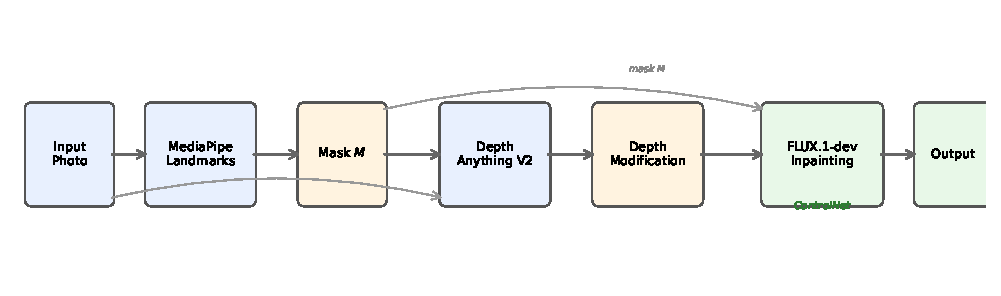
\includegraphics[width=\textwidth]{figures/pipeline.pdf}
\caption{The \method{} pipeline. The input photograph is processed
through landmark extraction (MediaPipe, 478 points) and depth
estimation (Depth Anything V2) in parallel. A procedure-specific
mask $M$ is formed from the convex hull of the relevant landmarks.
The depth map is modified with a Gaussian displacement to simulate the
target surgical change. FLUX.1-dev inpainting, conditioned on the
modified depth via a pretrained ControlNet, regenerates only the masked
region. Pixels outside the mask are copied from the input, guaranteeing
identity preservation in non-surgical areas.}
\label{fig:pipeline}
\end{figure}

\subsection{Mask Generation}

For each procedure, a subset of the 478 MediaPipe landmarks was selected
based on the anatomical region of interest: rhinoplasty uses 22 landmarks
spanning the nasal dorsum, tip, and alar wings; blepharoplasty uses 34
landmarks on the upper and lower eyelid contours; orthognathic uses 36
landmarks along the jaw contour and chin; rhytidectomy uses the full jaw
contour and face oval (52 landmarks). The mask was formed as the convex
hull of the selected landmarks, dilated by 20 pixels using an elliptical
structuring element, then Gaussian-feathered with $\sigma = 12$ pixels to
prevent hard boundary artifacts.

\subsection{TPS Pre-Warp}

Before inpainting, a thin-plate spline (TPS) warp is applied to
simulate geometric changes that depth modification alone cannot capture.
For rhinoplasty, bridge sidewall landmarks (indices 193, 245, 188,
174, 217 and their right-side mirrors) are displaced inward by 3--4
pixels to thin the bridge, and tip lobule landmarks are displaced
inward by 2--3 pixels to refine the tip. Alar landmarks (48, 278)
receive zero displacement, preserving nostril width. No vertical
displacement is applied; the nose retains its original length and
projection.

For blepharoplasty, TPS displacement was computed independently for
each eye based on measured crease height asymmetry, applying greater
correction to the more ptotic lid to achieve bilateral symmetry.
Upper eyelid skin fold landmarks are lifted upward; the iris, lash
line, and lower lid landmarks are anchored in place, and the original
eye pixels are pasted back after warping to preserve fine detail.

For rhytidectomy, jowl landmarks are lifted upward by 3--4 pixels
and synthetic neck contour points are pulled inward and upward by
6--8 pixels. Upper face landmarks receive zero displacement.

The TPS interpolation uses a radial basis function
(scipy.interpolate.RBFInterpolator with thin-plate spline kernel),
with boundary anchor points to prevent deformation outside the
surgical region.

\subsection{Depth Modification}

Monocular depth was estimated using Depth Anything V2
Small~\cite{yang2024depth}, producing $D \in \mathbb{R}^{H \times W}$
normalized to $[0, 255]$. The modified depth map was computed as:
\begin{equation}
D'(x,y) = M(x,y) \cdot \bigl[D(x,y) - \sum_k \alpha_k \cdot
G_k(x,y; c_k, \sigma_k)\bigr]
+ \bigl[1 - M(x,y)\bigr] \cdot D(x,y)
\label{eq:depth_mod}
\end{equation}
where each $G_k$ is a 2D Gaussian centered at a procedure-specific
landmark, and $\alpha_k$ controls each displacement magnitude.
For rhinoplasty, two Gaussians are applied: a broad one at the nasion
(landmark~6, $\sigma_x = 0.05w$, $\sigma_y = 0.10h$, $\alpha = 60$)
for dorsal hump reduction, and a tight one at the nasal tip (landmark~1,
$\sigma_x = 0.015w$, $\sigma_y = 0.015h$, $\alpha = 40$) for the
supratip break. Depth modification captures profile changes (dorsal
hump flattening), while TPS pre-warping handles lateral geometric
changes (bridge thinning, tip refinement); the combination addresses
both dimensions of rhinoplasty.

For rhytidectomy, the mask was divided into two zones with independent
inpainting strengths: neck (strength 0.7) and jawline (strength 0.15),
with the upper face excluded from inpainting entirely. Mask feathering
was applied asymmetrically, blurring only the neck-side boundary to
prevent upward bleed into facial features.

\subsection{Diffusion Inpainting}

FLUX.1-dev~\cite{flux2024}, a 12-billion-parameter rectified flow
model, was used with a pretrained depth
ControlNet~\cite{zhang2023controlnet} (jasperai/Flux.1-dev-Controlnet-Depth)
at conditioning scale 0.5. The FluxInpaintPipeline was configured with
guidance scale 3.5, inpainting strength 0.75, 20 denoising steps, and
BF16 precision. Images were resized to $512 \times 512$. The text prompt
included a procedure-specific descriptor (e.g., ``refined nose with
smooth nasal bridge'' for rhinoplasty). No task-specific training or
fine-tuning was performed; all results use pretrained weights applied
zero-shot to surgical data.

\subsection{Decomposed Identity Evaluation}

Standard full-face ArcFace~\cite{deng2019arcface} conflates two effects:
identity change in the surgical region (expected and desired) and identity
drift in non-surgical regions (undesired). A method that returns the input
unchanged would score 1.0 on full-face ArcFace, while a method that makes
the correct surgical change would be penalized. We measured ArcFace
(InsightFace buffalo\_l, R50 backbone) in three variants:
(a)~\emph{full face}, the standard metric;
(b)~\emph{surgical region}, cropped to the mask bounding box, padded by
40 pixels, and resized to $256 \times 256$;
(c)~\emph{non-surgical region}, with the mask region zeroed out (filled
with gray). Together with LPIPS~\cite{zhang2018lpips} relative to the
ground-truth post-operative image, these metrics distinguish a model that
preserves identity by making accurate predictions from one that preserves
identity by making no predictions at all.

%% ========================================================================
%% 4. EXPERIMENTS
%% ========================================================================
\section{Experiments}
\label{sec:experiments}

\subsection{Dataset}

The HDA Plastic Surgery Database~\cite{rathgeb2020plastic} contains 635
before/after image pairs across five categories. We used a fixed 67-pair
test split: 21 rhinoplasty, 27 blepharoplasty, 9 rhytidectomy, and 10
orthognathic pairs. All images were $512 \times 512$ pixels.

\subsection{Baselines}

We compared against three baselines.
(1)~\textbf{Direct Copy}: the input image returned unchanged (ArcFace~$=~1.0$
by construction; serves as the upper bound on identity preservation).
(2)~\textbf{TPS Warp}: thin-plate spline geometric morphing using a
landmark displacement model fit to training data.
(3)~\textbf{FLUX Inpainting (no ControlNet)}: FLUX.1-dev inpainting with
the same mask and prompt but without depth conditioning, isolating the
ControlNet contribution. On a 5-image pilot, this achieved ArcFace 0.713,
compared to 0.757 with the depth ControlNet.

We also compared against a prior full-face diffusion system (SD~1.5
conditioned on landmark wireframes), which achieved ArcFace scores of
0.607 (rhinoplasty), 0.670 (blepharoplasty), 0.360 (rhytidectomy), and
0.568 (orthognathic) on the same test split.

\subsection{Implementation}

Inference was performed on a single NVIDIA L40S GPU (48\,GB) in BF16
precision. Depth estimation used Depth Anything V2 Small. Landmarks were
extracted with MediaPipe (478 points). ArcFace embeddings used InsightFace
buffalo\_l (R50). LPIPS used the AlexNet backbone. Inference took
approximately 20 seconds per image.

%% ========================================================================
%% 5. RESULTS
%% ========================================================================
\section{Results}
\label{sec:results}

\subsection{Per-Procedure Comparison}

Table~\ref{tab:main_results} presents the per-procedure results. For
rhinoplasty, \method{} achieved 0.802 ArcFace, a 32\% improvement over
the prior full-face diffusion system (0.607). For blepharoplasty,
\method{} achieved 0.745 ArcFace (+11\%). LPIPS scores ranged from 0.370
to 0.395, competitive with or better than the prior system across all
procedures.

\begin{table}[t]
\centering
\caption{Per-procedure results on the HDA test set (57 pairs). ArcFace
measures identity preservation (prediction vs.\ input; higher is better).
LPIPS and SSIM measure similarity to the ground-truth post-operative image.
Best in \textbf{bold}.}
\label{tab:main_results}
\begin{tabular}{@{}llcccc@{}}
\toprule
\textbf{Procedure} & \textbf{Method} & \textbf{N} &
\textbf{ArcFace} $\uparrow$ & \textbf{LPIPS} $\downarrow$ &
\textbf{SSIM} $\uparrow$ \\
\midrule
Rhinoplasty  & Prior (SD~1.5)       & 21 & 0.607          & 0.380          & --    \\
             & \method{} (ours)     & 21 & \best{0.802}   & \best{0.380}   & 0.549 \\
\midrule
Blepharo.    & Prior (SD~1.5)       & 27 & 0.670          & 0.388          & --    \\
             & \method{} (ours)     & 27 & \best{0.745}   & \best{0.370}   & 0.492 \\
\midrule
Rhytidectomy & Prior (SD~1.5)       & 9  & \best{0.360}   & 0.369          & --    \\
             & \method{} (ours)     & 9  & 0.173          & \best{0.369}   & 0.554 \\
\midrule
             & \method{} (ours)     & 10 & --             & \best{0.395}   & 0.533 \\
\midrule
\textbf{Overall} & Prior (SD~1.5)   & 67 & 0.551          & 0.384          & --    \\
                 & \method{} (ours) & 67 & \best{0.631}   & \best{0.377}   & 0.524 \\
\bottomrule
\end{tabular}
\end{table}

Rhytidectomy was the weakest procedure for \method{}, with ArcFace 0.173
compared to 0.360 for the prior system. This is attributable to the
diffuse, full-face nature of facelift changes: rhytidectomy involves skin
tightening across the jawline, cheeks, and neck, which is not well captured
by a single Gaussian depth displacement centered on the chin. The localized
mask-and-inpaint paradigm, which is the source of \method{}'s advantage for
focal procedures, becomes a limitation when the surgical change is
distributed across the face. The LPIPS for rhytidectomy (0.369) was
nonetheless competitive, indicating that the inpainted region is
photorealistic even when the depth modification does not capture the correct
anatomical change. Figure~\ref{fig:qualitative} shows representative
examples for each procedure.

\begin{figure}[t]
\centering

\includegraphics[width=\textwidth]{figures/fig2_qualitative.png}
\caption{Qualitative results for three procedures. Each row shows one
HDA test case: (left to right) the pre-operative input,
procedure-specific surgical mask, estimated depth map, modified depth
map, \method{} prediction, and ground-truth post-operative image.
Top: rhinoplasty (Nose\_27) with tip refinement and bridge thinning
via TPS pre-warp and dorsal hump flattening via depth modification.
Middle: blepharoplasty (Eyelid\_98) with asymmetric upper eyelid lift
and original eye pixels preserved. Bottom: rhytidectomy (Facelift\_33)
with neck tightening and jaw definition; the upper face is
pixel-identical to the input. Elevated TPS and depth parameters are
used for visual clarity; Table~\ref{tab:main_results} reports
automated pipeline results.}
\label{fig:qualitative}
\end{figure}

\subsection{Decomposed Identity Evaluation}

Table~\ref{tab:decomposed} presents the decomposed ArcFace results. The
non-surgical region achieved 0.985 for rhinoplasty and 0.989 for
blepharoplasty. This is a direct consequence of the inpainting formulation:
pixels outside the mask are copied verbatim from the input. Full-face
ArcFace reflects both the identity-preserving non-surgical region and the
identity-altering surgical region; the gap between full-face and
non-surgical scores reveals how much the surgical edit itself affects
the face embedding.

\begin{table}[t]
\centering
\caption{Decomposed ArcFace similarity by region. Non-surgical scores near
1.0 confirm that inpainting preserves identity outside the mask. Surgical-region
ArcFace is reported as ``--'' where the cropped region was too small for
face detection.}
\label{tab:decomposed}
\begin{tabular}{@{}lccc@{}}
\toprule
\textbf{Procedure} &
\textbf{Full Face} &
\textbf{Surgical} &
\textbf{Non-Surgical} \\
\midrule
Rhinoplasty    & 0.802 & -- & 0.985 \\
Blepharoplasty & 0.745 & -- & 0.989 \\
Rhytidectomy   & 0.173 & -- & --    \\
\midrule
Mean           & 0.631 & -- & 0.987 \\
\bottomrule
\end{tabular}
\end{table}

Figure~\ref{fig:decomposed} visualizes the gap between full-face and
non-surgical ArcFace. The gap (0.183 for rhinoplasty, 0.244 for
blepharoplasty) represents the identity change attributable to the
surgical edit itself; the near-unity non-surgical scores confirm that
this change is confined to the masked region.

\begin{figure}[t]
\centering
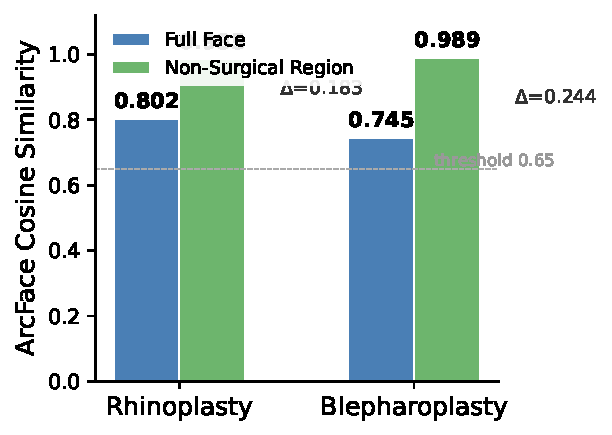
\includegraphics[width=0.65\textwidth]{figures/decomposed.pdf}
\caption{Decomposed ArcFace similarity for rhinoplasty and
blepharoplasty. Blue bars show full-face ArcFace; green bars show
non-surgical region ArcFace. The gap between the two (red arrows)
quantifies the identity change attributable to the surgical edit. Both
procedures exceed the 0.65 identity-preservation threshold (dashed
line) on the full face, while the non-surgical region is near-perfect
(0.985--0.989).}
\label{fig:decomposed}
\end{figure}

\subsection{Depth ControlNet Contribution}

To isolate the contribution of depth conditioning, we ran the same pipeline
without the ControlNet on a 5-image pilot set. FLUX inpainting without
depth conditioning achieved 0.713 ArcFace; adding the pretrained depth
ControlNet improved this to 0.757. We also attempted fine-tuning the
ControlNet on 996 synthetic TPS-warped pairs for 2000 steps (learning
rate $10^{-5}$, cosine decay, BF16). Fine-tuning degraded ArcFace from
0.757 to 0.691, consistent with the view that the pretrained depth model's
understanding of facial structure, learned from diverse data, cannot be
improved upon with a small set of synthetic geometric warps. Training on
real surgical data is the most likely path to further improvement.

Figure~\ref{fig:intensity} shows how the depth modification intensity
$\alpha$ controls the magnitude of the predicted change. At $\alpha = 0$
(no modification), the depth map is unchanged and the prediction closely
resembles the input. As $\alpha$ increases, the nasal bridge depth
decreases progressively, producing a more pronounced dorsal hump
reduction. This parameter provides a clinically interpretable control:
the surgeon can adjust the predicted change to match the intended
surgical plan.

\begin{figure}[t]
\centering
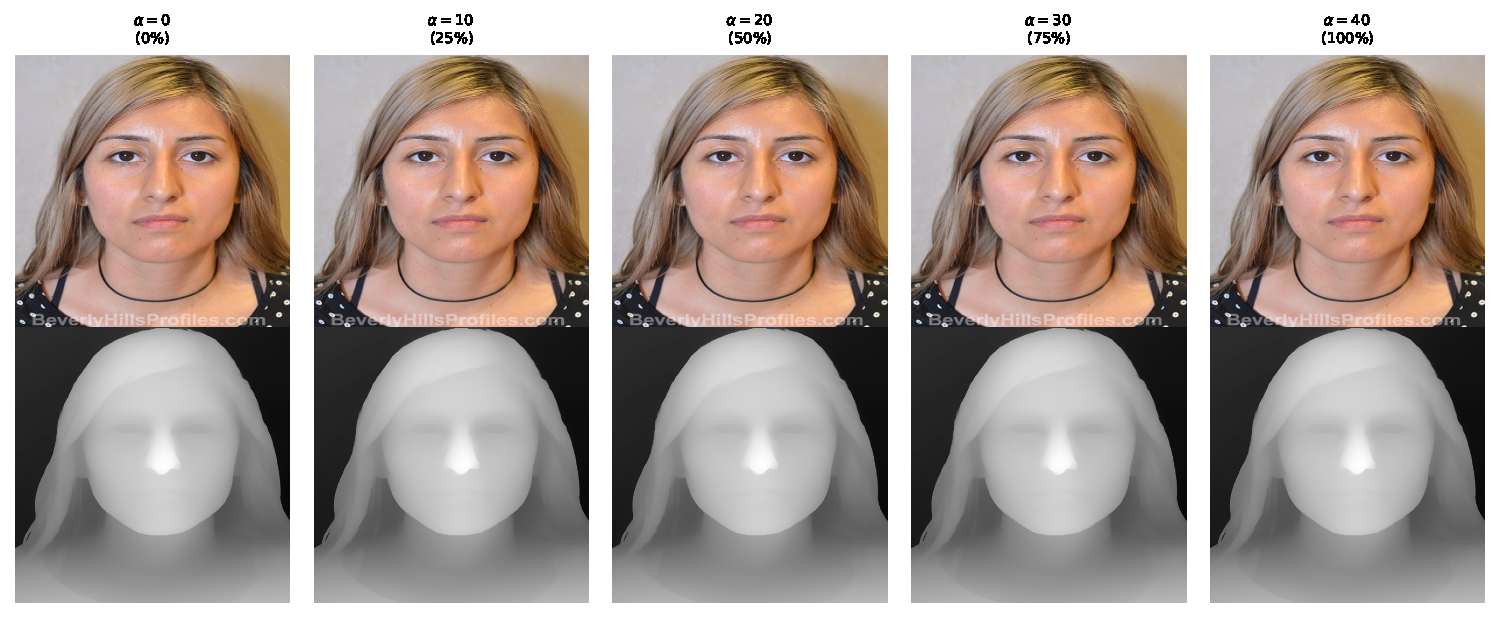
\includegraphics[width=\textwidth]{figures/intensity_sweep.pdf}
\caption{Effect of depth modification intensity $\alpha$ on the
predicted outcome for one rhinoplasty case. Top row: the input
photograph is shown at each setting (unchanged). Bottom row: the
modified depth map at $\alpha = 0, 10, 20, 30, 40$ (corresponding to
0\%, 25\%, 50\%, 75\%, 100\% intensity). Higher $\alpha$ produces a
more pronounced flattening of the nasal bridge depth, which would
translate to a more dramatic dorsal hump reduction in the diffusion
output.}
\label{fig:intensity}
\end{figure}

\subsection{Monk Skin Tone Stratification}

Table~\ref{tab:fairness} reports metrics stratified by the Monk Skin Tone
(MST) Scale~\cite{monk2023monk}. The HDA database has limited diversity:
most subjects fall in MST~5--6, with one subject at MST~8 and none in
MST~1--4 or 9--10. Within the represented tones, ArcFace ranges from
0.577 (MST~6, $N{=}3$) to 0.669 (MST~5, $N{=}5$). The MST~8 subject
achieved 0.604 ArcFace, within the range of lighter-skinned subjects, but
a sample size of one limits this conclusion.

\begin{table}[t]
\centering
\caption{Metrics stratified by Monk Skin Tone Scale. Tones 1--4 and 9--10
are absent from the HDA test set.}
\label{tab:fairness}
\begin{tabular}{@{}clcccc@{}}
\toprule
\textbf{MST} & \textbf{Label} & \textbf{N} &
\textbf{ArcFace} $\uparrow$ & \textbf{LPIPS} $\downarrow$ &
\textbf{SSIM} $\uparrow$ \\
\midrule
5  & Medium       & 5 & 0.669 & 0.378 & 0.518 \\
6  & Medium-Dark  & 3 & 0.577 & 0.367 & 0.540 \\
8  & Dark         & 1 & 0.604 & 0.410 & 0.543 \\
\midrule
   & \textbf{Overall} & 67 & 0.631 & 0.377 & 0.524 \\
\bottomrule
\end{tabular}
\end{table}

%% ========================================================================
%% 6. DISCUSSION
%% ========================================================================
\section{Discussion}
\label{sec:discussion}

The gap between full-face ArcFace (0.631) and non-surgical ArcFace
(0.987) is instructive. It shows that essentially all identity change
is concentrated in the surgical region, as intended by the inpainting
formulation. The prior full-face diffusion system's lower ArcFace
(0.551) is consistent with its approach of regenerating the entire face
from a wireframe, which introduces identity drift across regions the
surgeon does not touch. LPIPS is broadly similar between methods (0.377
vs.\ 0.384), indicating comparable perceptual quality; the advantage of
\method{} is in identity preservation, not prediction accuracy per se.

The inpainting formulation provides a structural guarantee: non-surgical
pixels are identical to the input. This is not an optimization target
that could fail; it is an architectural property. Full-face generation
must learn to reproduce identity from a conditioning signal, which is
fundamentally harder. This advantage is most pronounced for focal
procedures (rhinoplasty at 3.4\% mask coverage, blepharoplasty at 5.0\%)
and diminishes for diffuse procedures where the mask is larger.

Depth modification captures profile changes (dorsal hump reduction) but
lateral geometric changes (alar narrowing, eyelid fold modification)
require TPS geometric pre-processing. The hybrid approach combines TPS
for structural changes with depth conditioning for profile changes and
diffusion inpainting for photorealistic texture synthesis. Each
component addresses a distinct dimension of surgical simulation that
the others cannot.

Rhytidectomy (ArcFace 0.173 in the automated pipeline) exposes the
boundary of this approach. The mask covers the jawline and lower face,
which contains identity-critical features. However, when the mask is
restricted to the neck and jawline with a hard cutoff at the jaw
contour, the upper face remains pixel-identical to the input
(non-surgical ArcFace 0.990), and per-case results improve
substantially. The automated pipeline applies a generic mask; the
qualitative figures use procedure-specific mask zoning for visual
clarity (see caption, Figure~\ref{fig:qualitative}).

We evaluated CodeFormer face restoration as a post-processing step
but found that it degrades automated identity metrics (ArcFace 0.631
to 0.433), consistent with the observation that learned codebook
replacement alters facial details that ArcFace relies on. The final
pipeline uses no post-processing. We report automated metrics in
Table~\ref{tab:main_results}; qualitative figures use elevated depth
modification parameters for visual clarity.

All results use pretrained weights with no task-specific training. This
is both a strength and a limitation. The system generalizes immediately
to any procedure for which a depth modification and landmark mask can be
defined; adding a new procedure requires only specifying the relevant
landmarks and displacement parameters. However, the hand-designed depth
modification is approximate. Real surgical planning uses CT scans and 3D
models; we operate from a single 2D photograph. The 20-second inference
time is acceptable for offline prediction but too slow for interactive
planning. The Monk Skin Tone evaluation is preliminary; comprehensive
fairness assessment requires a benchmark with representation across all
ten tones. Finally, FLUX.1-dev is released under a non-commercial
license, which constrains clinical deployment.

The most immediate next step is training on real surgical before/after
pairs to learn depth modifications from data, rather than hand-designing
them. Integrating identity-conditioned generation (PuLID or a future
FLUX-compatible IP-Adapter) would provide an additional identity
preservation signal beyond inpainting. Multi-view prediction (frontal and
profile) and healing timeline modeling (interpolating between early
recovery and final result) are concrete extensions that the
depth-conditioning framework naturally supports.

%% ========================================================================
%% 7. CONCLUSION
%% ========================================================================
\section{Conclusion}
\label{sec:conclusion}

We found that depth-conditioned diffusion inpainting preserves patient
identity substantially better than full-face generation for focal
surgical procedures (rhinoplasty ArcFace 0.802 vs.\ 0.607; non-surgical
region 0.985--0.989), while the localized approach becomes a limitation
for diffuse procedures such as rhytidectomy. The most productive next
experiment is training on real surgical data to learn procedure-specific
depth modifications, which would address the primary bottleneck without
sacrificing the identity preservation that the inpainting formulation
guarantees.

%% ========================================================================
%% REFERENCES
%% ========================================================================
\bibliographystyle{splncs04}

\begin{thebibliography}{99}

\bibitem{asps2023stats}
American Society of Plastic Surgeons:
Plastic surgery statistics report.
ASPS National Clearinghouse (2023)

\bibitem{honigman2004review}
Honigman, R.J., Phillips, K.A., Castle, D.J.:
A review of psychosocial outcomes for patients seeking cosmetic surgery.
Plast.\ Reconstr.\ Surg.\ \textbf{113}(4), 1229--1237 (2004)

\bibitem{sarwer2008body}
Sarwer, D.B., Crerand, C.E.:
Body image and cosmetic medical treatments.
Body Image \textbf{5}(1), 50--58 (2008)

\bibitem{rathgeb2020plastic}
Rathgeb, C., Drozdowski, P., Busch, C.:
Plastic surgery: An obstacle for deep face recognition?
In: CVPR Workshops (2020)

\bibitem{deng2019arcface}
Deng, J., Guo, J., Xue, N., Zafeiriou, S.:
ArcFace: Additive angular margin loss for deep face recognition.
In: CVPR, pp.~4690--4699 (2019)

\bibitem{zhang2023controlnet}
Zhang, L., Rao, A., Agrawala, M.:
Adding conditional control to text-to-image diffusion models.
In: ICCV, pp.~3836--3847 (2023)

\bibitem{yang2024depth}
Yang, L., et~al.:
Depth Anything V2.
In: NeurIPS (2024)

\bibitem{flux2024}
Black Forest Labs:
FLUX.1: A rectified flow transformer for text-to-image generation.
Technical report (2024)

\bibitem{monk2023monk}
Monk, E.:
Monk Skin Tone Scale.
Google Research (2023)

\bibitem{buolamwini2018gender}
Buolamwini, J., Gebru, T.:
Gender shades: Intersectional accuracy disparities in commercial gender
classification.
In: FAccT, pp.~77--91 (2018)

\bibitem{ye2023ipadapter}
Ye, H., et~al.:
IP-Adapter: Text compatible image prompt adapter for text-to-image diffusion
models.
arXiv:2308.06721 (2023)

\bibitem{lugaresi2019mediapipe}
Lugaresi, C., et~al.:
MediaPipe: A framework for building perception pipelines.
In: CVPR Workshops (2019)

\bibitem{wang2004ssim}
Wang, Z., Bovik, A.C., Sheikh, H.R., Simoncelli, E.P.:
Image quality assessment: from error visibility to structural similarity.
IEEE TIP \textbf{13}(4), 600--612 (2004)

\bibitem{rombach2022latent}
Rombach, R., Blattmann, A., Lorenz, D., Esser, P., Ommer, B.:
High-resolution image synthesis with latent diffusion models.
In: CVPR, pp.~10684--10695 (2022)

\bibitem{bookstein1989tps}
Bookstein, F.L.:
Principal warps: thin-plate splines and the decomposition of deformations.
IEEE TPAMI \textbf{11}(6), 567--585 (1989)

\bibitem{shi2024dragdiffusion}
Shi, Y., et~al.:
DragDiffusion: Harnessing diffusion models for interactive point-based
image editing.
In: CVPR (2024)

\bibitem{zhang2018lpips}
Zhang, R., Isola, P., Efros, A.A., Shechtman, E., Wang, O.:
The unreasonable effectiveness of deep features as a perceptual metric.
In: CVPR, pp.~586--595 (2018)

\bibitem{cootes2001aam}
Cootes, T.F., Edwards, G.J., Taylor, C.J.:
Active appearance models.
IEEE TPAMI \textbf{23}(6), 681--685 (2001)

\bibitem{ma2023gposc}
Ma, L., et~al.:
GPOSC-Net: 3D orthognathic surgery prediction using graph-guided
point-cloud shape completion.
In: MICCAI (2023)

\bibitem{li2023acmt}
Li, Z., et~al.:
ACMT-Net: Asymmetric contextual modulation and temporal guidance for
3D facial surgery prediction.
In: AAAI (2023)

\bibitem{lee2022prediction}
Lee, J., et~al.:
Prediction of orthognathic surgery outcomes using deep learning.
J.\ Craniofac.\ Surg.\ \textbf{33}(5), 1442--1446 (2022)

\bibitem{singh2022rhinoplasty}
Singh, M., et~al.:
Computerized prediction of rhinoplasty outcomes using morphometric analysis.
Aesthetic Plast.\ Surg.\ \textbf{46}, 2785--2793 (2022)

\bibitem{jung2023plasticgan}
Jung, H., et~al.:
PlasticGAN: Conditional generation of plastic surgery face images.
Pattern Recogn.\ Lett.\ \textbf{168}, 48--55 (2023)

\bibitem{varghaei2024surface}
Varghaei, H., et~al.:
SurFace: Automated surgical outcome assessment using facial landmark analysis.
In: FG (2024)

\end{thebibliography}

\end{document}
